\documentclass[PI,KR]{HSEUniversity}
% Возможные опции: KR или VKR; PI или BI

\title{Разработка Информационной системы для поиска исполнителей по техническому заданию прикладного проекта}
\author{Соломатин Роман Игоревич}
\supervisor{к.т.н., доцент кафедры Информационных технологий в бизнесе НИУ ВШЭ-Пермь}{А. В. Бузмаков}
\Year{2021}
\Abstract{
	После титульного листа размещается краткая (до 0,5 стр.) аннотация, предназначенная для реферативных изданий (например, журналы ВИНИТИ) и библиотечных информационных систем. В ней перечисляются автор, наименование работы; о чем она написана и для кого; количество страниц, иллюстраций, год, издательство (в данном случае – кафедра). Пример аннотации можно увидеть в любой книге на обороте титульного листа. Аннотации работ используются при формировании каталога работ, выполненных на кафедре. Текст аннотации оформляется в соответствии с правилами оформления основного текста работы.
}

% Ссылка на файл с описание библиографии
\bibliography{library.bib}


\begin{document}

% Обязательные элементы оформления: заголовочный слайд, аннотация, оглавление
\maketitle

\chapter*{Введение}

Задача поиска исполнителей очень актуальна для многих сфер жизни. В каждой компании появляется много заданий и не понятно, кто лучше с ними справится. Поиск исполнителей необходим для того, чтобы как можно более эффективно использовать ресурсы. 

Объект исследования - .

Предмет исследования - .

Цель работы – создать информационную систему для поиска исполнителя по техническому заданию.

Для достижения поставленной цели надо сделать:

Во второй главе описание проектирования системы.
В третьей главе .

\chapter{Анализ предметной сферы}
\section{Обзор существующих решений}
Не существует решений, которые реализовывали поиск компетенций сотрудников и подбирали для них задания. Поэтому надо создать такой продукт, который будет делать это.

Данная система поможет автоматизировать процессы:
\begin{itemize}
	\item Определения компетенций сотрудника
	\item Поиск сотрудников для выполнения задания
\end{itemize}
\begin{FIGURE}[h]{Автоматизация бизнес-процесса "Подбор сотрудника для проекта" \label{fig:example-figure-2}}
	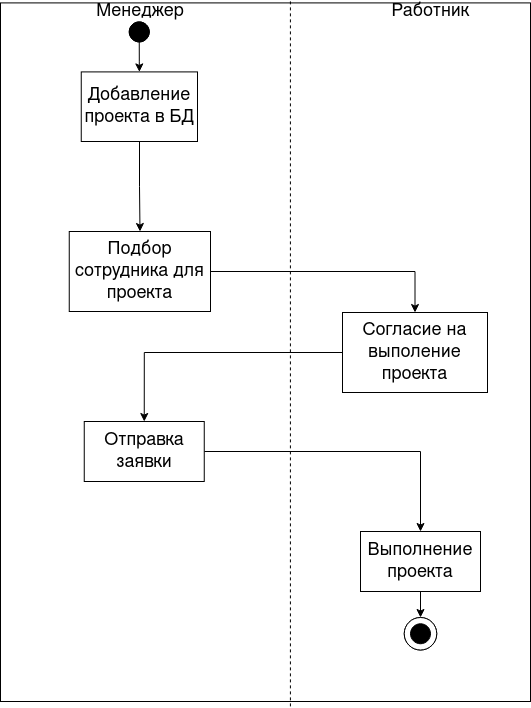
\includegraphics[width=0.4\textwidth]{img/Диаграмма Бизнес-процесса}
\end{FIGURE}
Варианты использования реализуемой системы:
\begin{itemize}
	\item Просмотр активных проектов
	\item Поиск компетенций работника
	\item Подбор сотрудника для проекта
	\item Редактирование информации о работнике
\end{itemize}

\begin{FIGURE}[h]{Диаграмма вариантов использования \label{fig:example-figure-2}}
	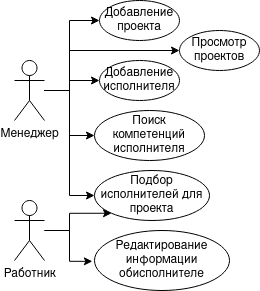
\includegraphics[width=0.4\textwidth]{img/Диаграмма вариантов использования}
\end{FIGURE}

\section{Выбор языка программирования}
При написании курсовой работы был выбор между двумя языками программирования C\# и Python. Основными критериями для выбора языка были:
\begin{itemize}
	\item Библиотеки для обучения моделей. Для работы с моделями машинного обучения.
	\item Предобученные модели. Так как для обучения модели надо иметь большой объем данных и много вычислительных мощностей.
\end{itemize} 

Для языка C\# есть фреймворк ML.NET, но для него мало библиотек и предобученных моделей.

Для Python есть фреймворк PyThorch и библиотека с предобученными моделями HuggingFace Transformers, а также есть библиотека Bert Extractive Summarizer \cite{miller2019leveraging}для удобной работы с моделей.

\section{Выбор СУБД}
В качестве системы управления базами данных был выбран SQLite. Так как для него библиотека входит в стандартную библиотеку Python и он занимает места.
\chapter{Проектирование системы}
\section{База данных}
Для хранение информации о преподавателях и выпускных квалификационных работах, где они были руководителями была разработана база данных. Необходимо было хранить:
\begin{itemize}
	\item Код преподавателя
	\item ФИО преподавателя
	\item Ссылка на профиль на сайте ВШЭ	
	\item Статус преподавателя
	\item Компетенции
	\item Эмбединги компетенций преподавателя
	\item Код статуса преподавателя
	\item Статус преподавателя (Старший преподаватель, доцент и тд.)
	\item Код факультета
	\item Факультет
	\item Код кафедры
	\item Кафедру
	\item Код ВКР
	\item Название ВКР
	\item Ссылку на ВКР на сайте ВШЭ
	\item Ссылку на текст ВКР
	\item Образовательную программу студента
	\item ФИО студента
\end{itemize} 
\subsection{Приведение к 1НФ}
Отношение находится в первой нормальной форме, если выполнены все свойства реляционных отношений, в частности все атрибуты отношения принимают простые значения (атомарные или неделимые), не являющиеся множеством или кортежем из более элементарных составляющих, все кортежи уникальны (отсутствуют дубли).

Данные атрибуты находятся в 1НФ.
\subsection{Приведение к 2НФ}
Отношение находится во второй нормальной форме, если оно находится в первой нормальной форме и каждый неключевой атрибут функционально полно зависит от всего ключа в целом, то есть отсутствует частичная функциональная зависимость не ключевых атрибутов от ключа.
\begin{itemize}
	\item Код преподавателя определяет:
	\begin{itemize}
		\item ФИО преподавателя
		\item Ссылка на профиль на сайте ВШЭ	
		\item Статус преподавателя
		\item Кафедра
		\item Компетенции
		\item Эмбединги компетенций преподавателя
		\item Код статуса преподавателя
	\end{itemize}
	\item Код статуса преподавателя определяет:
	\begin{itemize}
		\item Статус преподавателя
	\end{itemize}
	\item Код факультета определяет:
	\begin{itemize}
		\item Факультет
	\end{itemize}
	\item Код кафедры определяет:
	\begin{itemize}
		\item Кафедру
	\end{itemize}
	\item Код образовательной программы определяет:
	\begin{itemize}
		\item Название образовательной программы
	\end{itemize}
	\item ВКР определяет:
	\begin{itemize}
		\item Название ВКР
		\item Ссылку на ВКР на сайте ВШЭ
		\item Ссылку на текст ВКР
		\item Образовательную программу студента
		\item ФИО студента
		\item Преподавателя
		\item Образовательная программа
	\end{itemize}
\end{itemize}
\subsection{Приведение к 3НФ}
Отношение находится в третьей нормальной форме, если оно находится во второй нормальной форме, и каждый неключевой атрибут не является транзитивно зависимым от первичного ключа.
\section{Получение компетенций}
Для получение компетенций преподавателя использовались тексты ВКР, которые у него писали студенты. Для этого обрабатывался сайты Высшей школы экономики и скачивались тексты ВКР. Потом эти тексты группировались по преподавателю и обрабатывались с помощью Bert. 
\chapter{Разработка системы}


\putbibliography %Вместо этой команды будет вставлена библиография

\chapter*{Приложения}
\end{document}
